\begin{appendices}

\chapter{Lista defectelor din suită}
\label{apx:defecte}

\begin{figure}[h]
    \centering
    \caption{\centering Lista defectelor din suită (A)}
    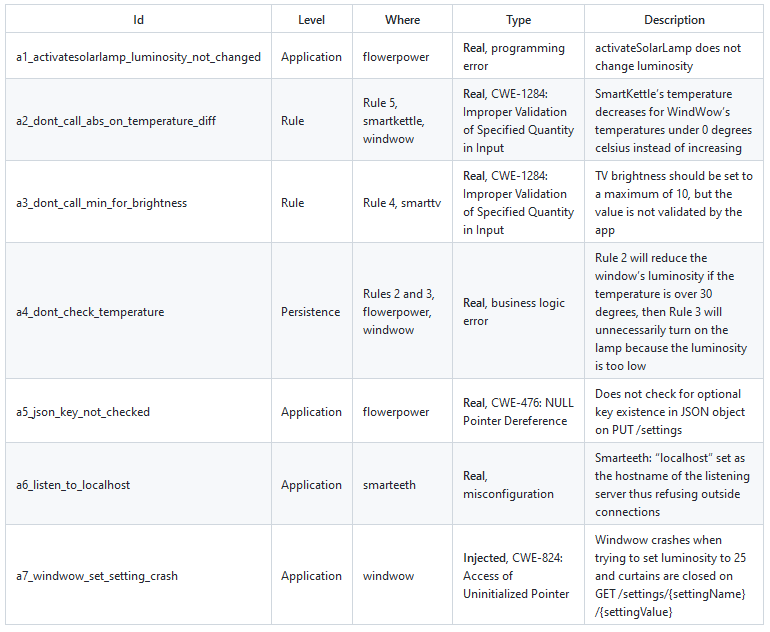
\includegraphics[width=0.9\textwidth]{images/tabel_bug2.png}
    \label{fig:tabel_bug1}
\end{figure}

\begin{figure}[h]
    \centering
    \caption{\centering Lista defectelor din suită (B)}
    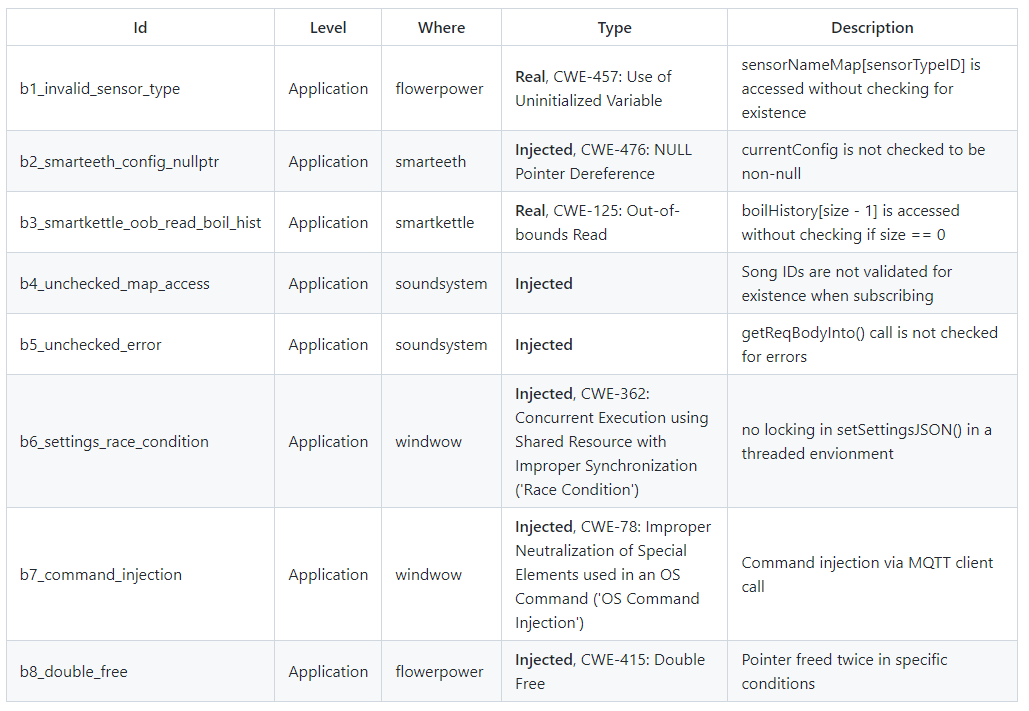
\includegraphics[width=0.9\textwidth]{images/tabel_bug1.png}
    \label{fig:tabel_bug2}
\end{figure}

\chapter{Ilustrații suplimentare}
\label{apx:ilustratii}

\begin{figure}[h]
    \centering
    \caption{\centering Modelul conceptual Open Systems Interconnection \newline (imagine prealuată de pe Wikipedia)}
    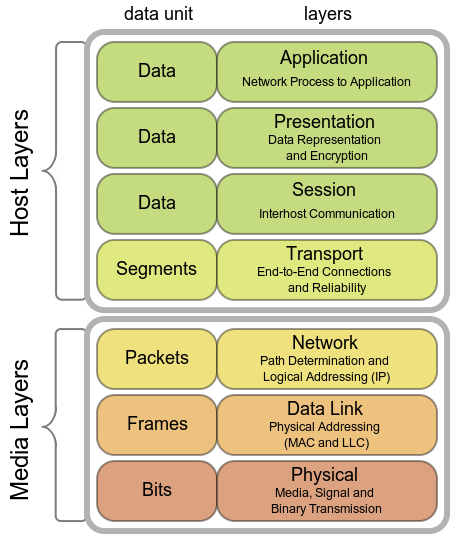
\includegraphics[width=0.8\textwidth]{images/OSI_Model_v1.png}
    \label{fig:osi_model}
\end{figure}

\begin{figure}[h]
    \centering
    \caption{Exemple de topologii ZigBee}
    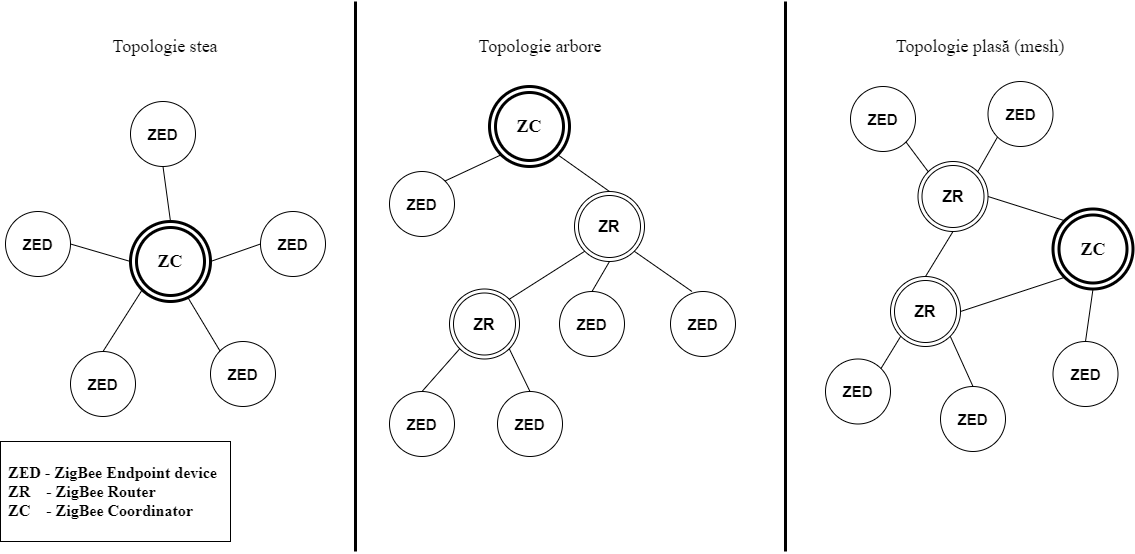
\includegraphics[width=0.9\textwidth]{images/topologii.drawio.png}
    \label{fig:zigbee_networks}
\end{figure}

\end{appendices}